\section{Literature Review}
\label{sec:review}

\subsection{Introduction}
The majority of mobile platforms or unmanned vehicles in use today are non-holonomic.
They only have one or two degrees of freedom that are independent. As a result, their
manoeuvrability is limited, and frequently require a large amount of space to control
functions such as turning and parking \cite{sheridan_telerobotics_1992}. This is apparent when an automobile wants to make a $180^0$ turn.
By increasing a vehicle’s degrees of freedom its manoeuvrability is greatly improved. It can follow many complex trajectories that conventional non-holonomic vehicles find difficult or impossible. Holonomic refers to the relationship between controllable and total degrees of
freedom of a robot. A holonomic platform is any mobile platform with three independent
degrees of freedom in a plane. If the controllable degree of freedom is equal to the total
degrees of freedom, then the robot is said to be holonomic \cite{titan_robotics_vision_and_control_fundamental_nodate}. Independent degrees of freedom indicate that it can change its orientation or position without affecting other motions, as
opposed to car-type vehicles, which must turn or change their orientation when moving.
A robot built on castor wheels or Omni-wheels is a good example of a holonomic drive as it can freely move in any direction and the controllable degrees of freedom are equal to total degrees of freedom. Holonomic drive makes a robot omnidirectional, meaning that the robot can move in any direction, forward/backwards but also sideways left/right, and turn on the spot, thanks to its wheels, giving the robot omnidirectional capabilities for movement on the horizontal axis on a drivetrain, as well as forward and backward movement \cite{robotics_omnidirectional_2022}.

\subsection{Mobile Robots}
There are different iterations of mobile robots, categorized into three broad categories - ground vehicles, underwater vehicles and aerial vehicles. This research narrows its focus to unmanned ground vehicles. \ac{UGVs} are robotic systems that operate on land without an onboard human operator \cite{rees_unmanned_nodate}. They are used for a wide variety of both civilian and military applications, particularly in environments that are hazardous or unpleasant to humans and for tasks that are difficult, dull or pose unacceptable risks. The three main locomotion methods for ground mobile robots are wheels, tracks and legs \cite{rees_unmanned_nodate}. Wheels are power-efficient and allow the highest speeds on flat ground, but are not good for traversing off-road and uneven terrain, as they can get stuck or sink into the ground due to low contact surface area and thus higher pressure. Tracks are the best option for rugged terrain but are slower, less efficient, involve more mechanical complexity and cause more vibration. Legged ground robots can cope with a wide variety of terrain, but are limited in speed and require complex control and stability hardware.

\begin{figure}[H]
    \centering
    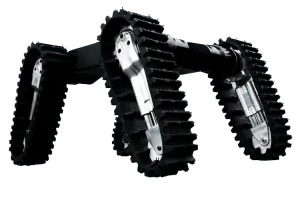
\includegraphics{Figures/ASI-Chaos-Unmanned-Vehicle.jpg}
    \caption{Tracked Ground Vehicle}
    \label{fig:trackedGV}
\end{figure}

For unmanned ground robots, wireless communication is used to relay sensor data and control instructions. \ac{UGVs} can be equipped with a variety of sensors and payloads. Due to operating in indoor and other environments deprived of the  \ac{GNSS}, \ac{UGVs} may rely on \ac{LiDAR} sensors, combined with inertial navigation systems and vehicle odometry, for accurate navigation\cite{rees_unmanned_nodate}. Mission-specific sensors and payloads include RGB and thermal cameras, manipulator arms, chemical and explosives sensors, and weapons systems\cite{rees_unmanned_nodate}. Consequently, unmanned ground vehicles have found applications in commercial and non-commercial use, including the military, firefighting, crowd control and in agriculture.


\subsection{Caster Wheel}
A castor or caster wheel is a relatively free-rolling, non-powered, small un-driven wheel.
It is designed for attachment to the bottom of a larger object, thus enabling easy movement across a floor or other hard surfaces. Caster wheels are manufactured in either a
single-wheel, double-wheel, or compound-wheel configuration.
Most castors are used simply to make a heavy or cumbersome piece of furniture or machinery - the vehicle - easier to move. Affixing small, unobtrusive wheels to the bottom
of any large or bulky item is a great way to make it more mobile in certain scenarios. In
most cases, they are attached to the underside of the vehicle via a fixed top plate, from
which the wheel assembly hangs. The caster wheel, through this attachment, has omnidirectional motion based on user input. It can move forward, backward and sideways in any direction and provides at least four degrees of freedom. 

\subsection{Existing Technologies and Research}
\subsubsection{Mecanum Wheels}
 Mecanum wheels achieve holonomic and omnidirectional motion by having a series of rollers attached to their circumference \cite{diegel_improved_nodate}. These rollers have an axis of rotation at 450
to the plane of the wheel. The angled peripheral rollers translate
a portion of the force in the rotational direction of the wheel \cite{diegel_improved_nodate}. Each mecanum wheel in a drive system has independent actuation and the resulting combination of forces to move these wheels produces a total force vector that allows the platform to move freely
in any direction. Different variations of mecanum wheels depend on the number of rollers attached to individual wheels, as shown in 
\ref{fig:differentvariationsofmecanumwheels}.

\begin{figure}[H]
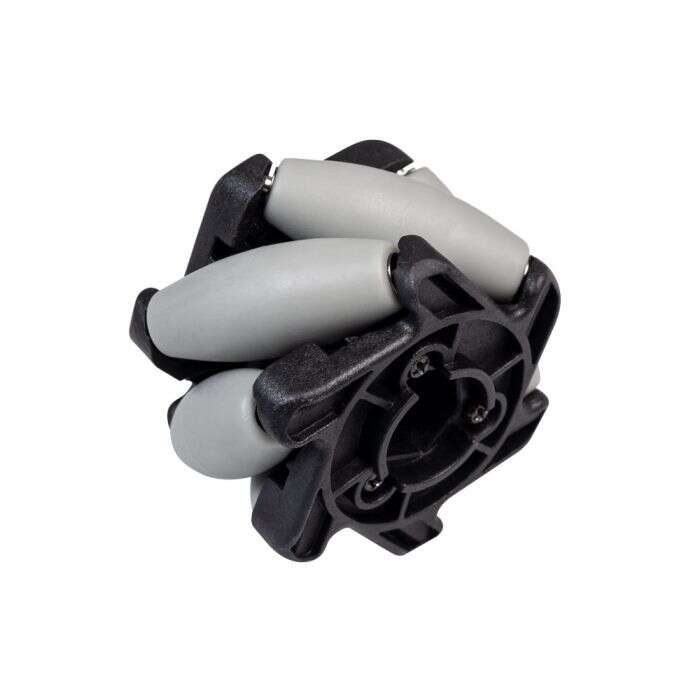
\includegraphics[scale=0.35]{Figures/mecanum1.jpg} 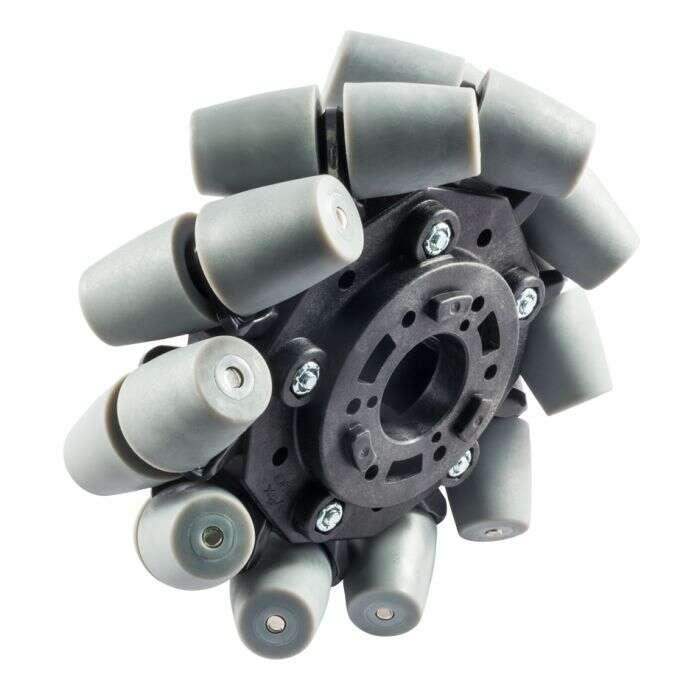
\includegraphics[scale=0.35]{Figures/mecanum2.jpg} 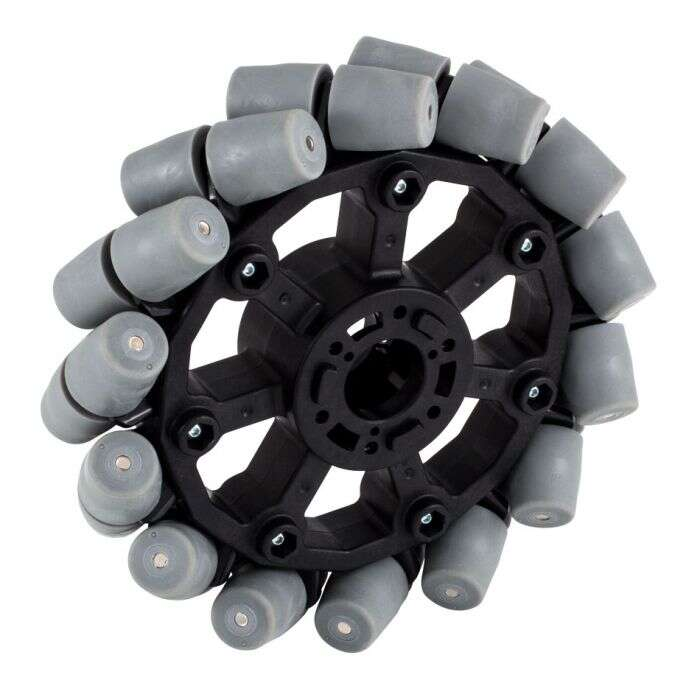
\includegraphics[scale=0.35]{Figures/mecanum3.jpg}\centering
\caption[Different variations of mecanum wheels] {Different variations of mecanum wheels \cite{diegel_improved_nodate}.}
\label{fig:differentvariationsofmecanumwheels}
\end{figure}

In the development of mecanum and other omnidirectional wheels \cite{kim_design_2001}\cite{rees_unmanned_nodate}, undesirable
vibrations are frequently present in the motion due to a large number of small rollers on the wheel’s periphery.

\subsubsection{Onidirectional and Holonomic Motion}
A lot of research and design work on omnidirectional vehicles has been conducted over the years.
The earliest omnidirectional mobile vehicle to be proposed was based on introducing a methodology for the kinematic modelling of an omnidirectional wheeled mobile robot equipped with four omnidirectional wheels which were based on passive rollers arranged in an overlapping way \cite{moreno_design_2016}. These wheels were positioned in pairs on the same axle but with opposite orientations. Another proposal by Wada and Mori \cite{wada_holonomic_1996} presented a new type of holonomic mobile robot which was equipped with steerable and coordinated driving wheels using conventional tires to provide an omnidirectional capability by actuating the wheels axis and a steering axis independently. In another paper by Javier Moreno, Eduard Clotet, and others designed a three-wheel holonomic motion system for an assistant personal robot \cite{moreno_design_2016}. The paper analyzes the kinematics of the motion system and validates the estimation of the trajectory by comparing the displacement estimated with the internal odometry of the motors and the displacement estimated with a \ac{SLAM} procedure based on \ac{LiDAR} information.

\subsubsection{Remote Control Strategies}
Remote control strategies refer to the methods and technologies used to remotely operate a device or system from a distance. These strategies are commonly used in various applications, including industrial automation, robotics, and military operations. In the context of mobile platforms, remote control strategies can be used to remotely operate and control the movement of the platform.

One commonly used remote control strategy for mobile platforms is the use of wireless communication technologies, such as Bluetooth, Wi-Fi, and radio frequency (RF) communication. These technologies allow the remote operator to send commands to the platform and receive feedback from the platform through a wireless connection. Wireless communication technologies have the advantage of being easy to set up and use, as well as being relatively inexpensive. However, they can be prone to interference and have limited range.

Another remote control strategy for mobile platforms is the use of remote control devices, such as joysticks, game controllers, and hand motion control devices. These devices allow the operator to control the movement of the platform through physical input, such as pressing buttons or moving a joystick. Remote control devices have the advantage of providing a more intuitive and immersive experience for the operator, as they can directly control the movement of the platform. However, they may require training and practice to use effectively, and may not be suitable for all applications.

Another remote control strategy for mobile platforms is the use of computer-based control systems, such as programmable logic controllers (PLCs) and industrial control systems (ICS). These systems allow the operator to remotely control the platform through a computer interface, using software programs and algorithms to control the movement of the platform. Computer-based control systems have the advantage of being highly flexible and customizable, as they can be programmed to perform a wide range of tasks. However, they may require specialized knowledge and expertise to set up and use, and may be more complex and expensive compared to other remote control strategies.

 The operator controls the remote robot with the control device while keeping an eye on the monitor, which displays visual data from the visual sensors. Expert operators who understand and are capable of training the remote-controlled robot are required to operate it flexibly. Thus, operating a remote-controlled robot is difficult and may result in operational errors. This is because using a monitor that only displays visual information makes it difficult for the operator to understand real-world environmental situations. As a result, numerous stages of training are required for the operator to recognise the surroundings from visual information for expert operation \cite{masaki_remote-controlled_2022}. Methods for improving the operability of the remote-controlled robot in terms of the mechanical design of the control device and the operation-assist control method have been discovered. Wireless control strategies have advanced the multi-operability of robots \cite{almali_wireless_nodate} but they are just a network to which control strategies connect. This study proposes a remote-controlled method with an \ac{API} to improve the diversity of remote-control applications.

\subsection{Gap Analysis}
Huge leaps have been made in the development of mobile vehicles or robots with holonomic and omnidirectional motion. Mecanum wheels have taken centre stage, and the use of rollers attached to a conventional wheel has found great applications in small-scale robots and mobile platforms. However, these wheels cannot be applied to certain applications that involve heavy payloads or rough terrains. Such applications are moving objects in warehouses or factory floors. Castors are predominantly used in these areas, but they have to be manually controlled. This process can be automated by modifying the castors through adding motors for directional control and adding the concept of remote control. Furthermore, robots have lacked the design of \ac{API}s embedded in their control. Most robots, if not all, have a fixed mode of control. This project seeks to explore how \ac{API}s can be added to robot control.

















